\chapter{Problem Specification}

In this chapter we will introduce the graph optimisation problem and establish the baseline performance using cost-based backtracking optimisation. Next, we will frame the optimisation problem in the RL domain by describing the system environment, the reward calculation and the state-action space. Additionally, we describe the RL agents trained in the model-free and model-based domains and we also highlight limitations in the application of reinforcement learning to this problem.

\section{Introduction}
The major deep learning frameworks such as TensorFlow \cite{tensorflow2015-whitepaper} and PyTorch \cite{pytorch} used greedy rule-based graph transformation prior to execution. Furthermore, in Chapter \ref{sec:bg:subsec:currentapp} we described the prior work upon which this work builds. Namely, we introduced the work by Jia et al. \cite{jia2019taso,jia2019optimizing} that proposed an approach for performing an offline optimisation of deep learning computation graphs using a recursive backtracking search in the action space. Specifically, the authors developed a framework that uses a pre-generated set of formally verified, semantically equivalent graph substitutions that can be used to modify the graph to search for a reduced runtime.

\section{Optimisation of deep learning graphs}

TensorFlow (TF) uses a system called \textit{``Grappler''} that is the default graph optimisation system in the TF runtime \cite{larsen2019tensorflow}. By natively performing the graph optimisation at runtime, it allows for a interoperable, transparent optimisation strategy via protocol buffers. To improve the performance of the underlying model, Grappler supports a range of features such as the pruning of dead nodes, removal of redundant computation and improved memory layouts. Concretely, Grappler was designed with three primary goals:

\begin{itemize}
  \item Automatically improve performance through graph simplifications and high-level optimisations to benefit the most target architectures
  \item Reduce device peak memory usage
  \item Improve hardware utilisation by optimising device placement
\end{itemize}

On the other hand, although Grappler can automatically optimise the data-flow graphs of deep learning models, such a complex optimisation system presents challenges. Firstly, significant engineering effort is required to implement, verify and test the optimiser to ensure the correctness of the graph rewrites rules; TF contains a set of 155 substitutions that are implemented in 53,000 lines of code; to further complicate matters, new operators are continuously proposed, such as grouped or transposed convolutions, all of which leads to a large amount effort expended to maintain the library. Secondly, and perhaps more importantly, as TF uses Grappler at runtime by default, it adds overhead to execution as extra graph conversions are performed at runtime rather than offline.

\begin{figure}[ht]
  \centering
  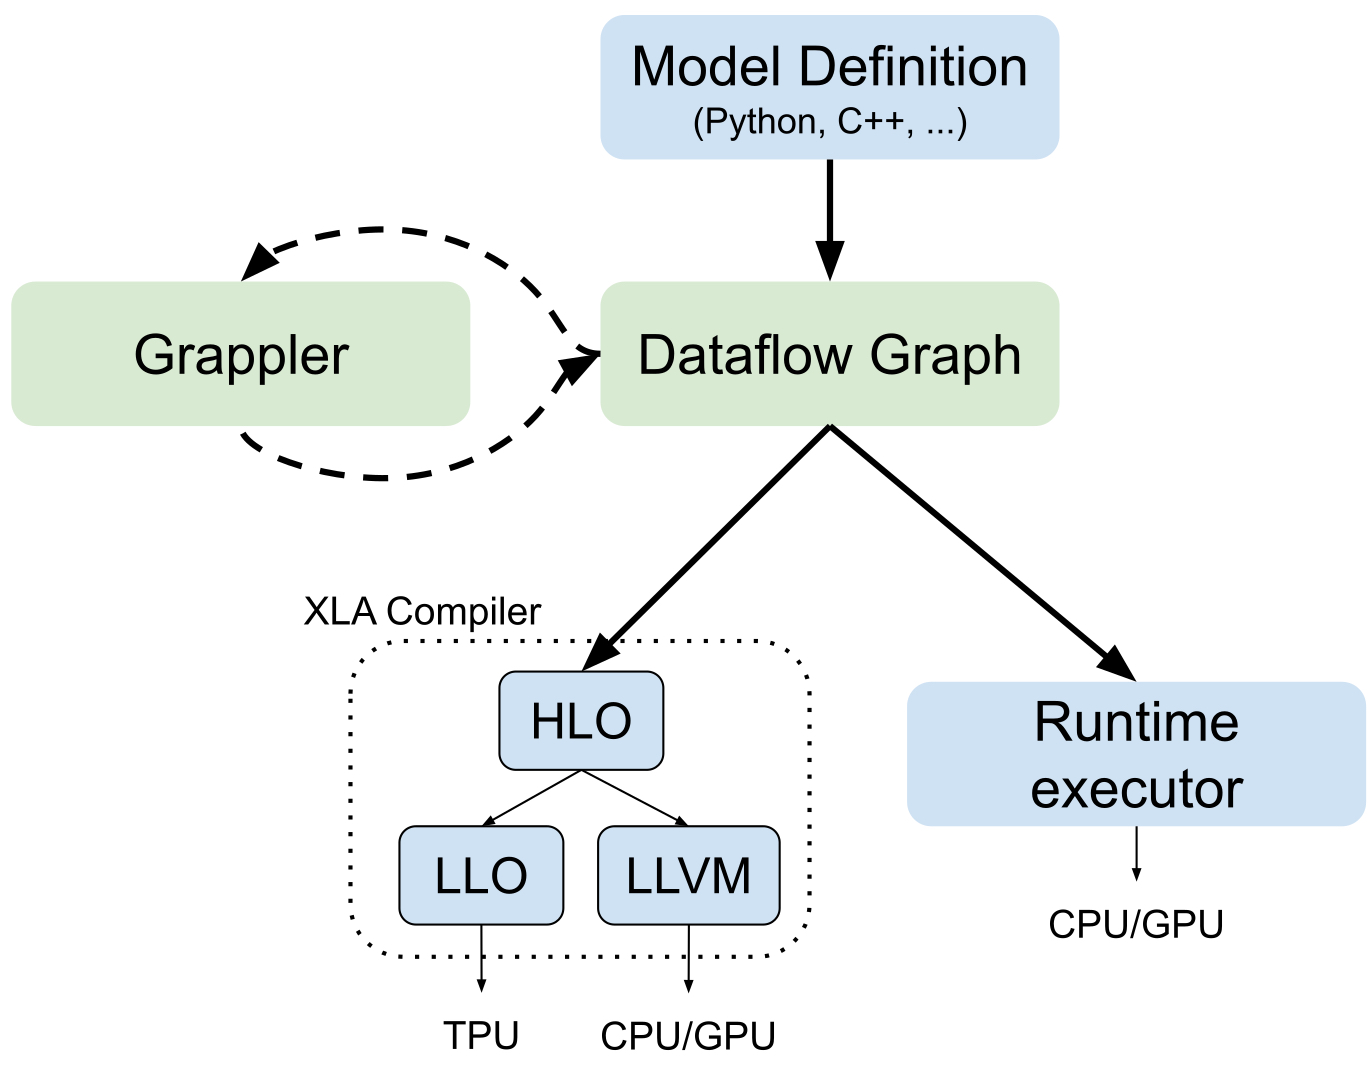
\includegraphics[width=0.75\columnwidth]{sections/3problem/images/GraphOptimiser.jpg}
  \caption[Architecture of graph optimisation system in TensorFlow]{The machine learning model is processed prior to execution by either Grappler, the static graph optimiser in TensorFlow, or via JIT compilation of the model using XLA. Figure adapted from \cite{larsen2019tensorflow}.}
  \label{fig:problem:graph-optim}
\end{figure}

Alternatively, both TensorFlow, and more recently PyTorch, support automatic graph optimisation by JIT (just-in-time) compilation through XLA and the \texttt{torch.jit} package respectively. In Figure \ref{fig:problem:graph-optim} we can see a high-level view of the components of the optimisation system. In order to motivate the reasoning to perform offline optimisation rather than JIT optimisation we  consider the work proposed by Jia et al. in both MetaFlow and TASO, the systems they design can be used as a drop-in replacement of the Grappler and/or XLA compilation steps.

TASO applies all possible candidate transformations at each step and estimates the runtime (or cost) of the final graph. Next, TASO chooses the highest performing candidates for the proceeding iteration of candidate evaluations. Principally, this approach is superior to the naive greedy optimisation approach as we can use the estimated runtime to guide the search and forego immediate improved runtime to increase the potential search space of candidate graphs.

In addition, as TASO operates at the graph-level, its optimisations are completely orthogonal to operator-level optimisations; thus it can be combined with code generation techniques such as TVM \cite{chen2018tvm} or Astra \cite{sivathanu2019astra} to further improve overall performance. We also note that TASO performs tensor data layout and graph transformation simultaneously rather than sequentially. It has been shown that by considering it as a joint optimisation problem end-to-end inference runtime can be reduced by up to 1.5x \cite{jia2019taso, jia2019optimizing}.

% However, using estimated runtime presents a challenge with respect to the exponential growth of search space at a rate of $O(N^T)$, where $N$ is the number of transformations and $T$ is the number of search steps.

\subsection{Graph-level optimisation}

Performing optimisations at a higher, graph-level means that the resulting graph is - in terms of execution methodology - no different than the original graph prior to optimisation. Therefore, by performing graph-level optimisation we generate a platform and backend independent graph representation which can be further optimised by specialised software for custom hardware accelerators such as GPUs and TPUs.

Next, we define that two computation graphs, $\mathcal{G}$ and $\mathcal{G}'$ are semantically equivalent when $\forall \mathcal{I} : \mathcal{G}(\mathcal{I}) = \mathcal{G}'(\mathcal{I})$ where $\mathcal{I}$ is an arbitrary input tensor. We aim to find the optimal graph $\mathcal{G}^*$ that minimises the cost function, \texttt{cost}$(\mathcal{G})$, by performing a series of transformations to the computation graph - at each step, the specific transformation applied does not need to be strictly optimal. In fact, by applying optimisations that reduce graph runtime we further increase the state space for the search; a large state space is preferable in the reinforcement learning domain.

An important problem in graph-level optimisation is that of defining a set of varied, applicable transformations that can be used to optimise the graphs. As previously noted, prior work such as TensorFlow use a manually defined set of transformations and optimise greedily. On the other hand, TASO uses a fully automatic method to generate candidate transformations by performing a hash-based enumeration over all possible DNN operators that result in a semantically equivalent computation graph.


\begin{figure}[ht]
  % preliminary
  \sbox\twosubbox{%
    \resizebox{\dimexpr.9\textwidth-1em}{!}{%
      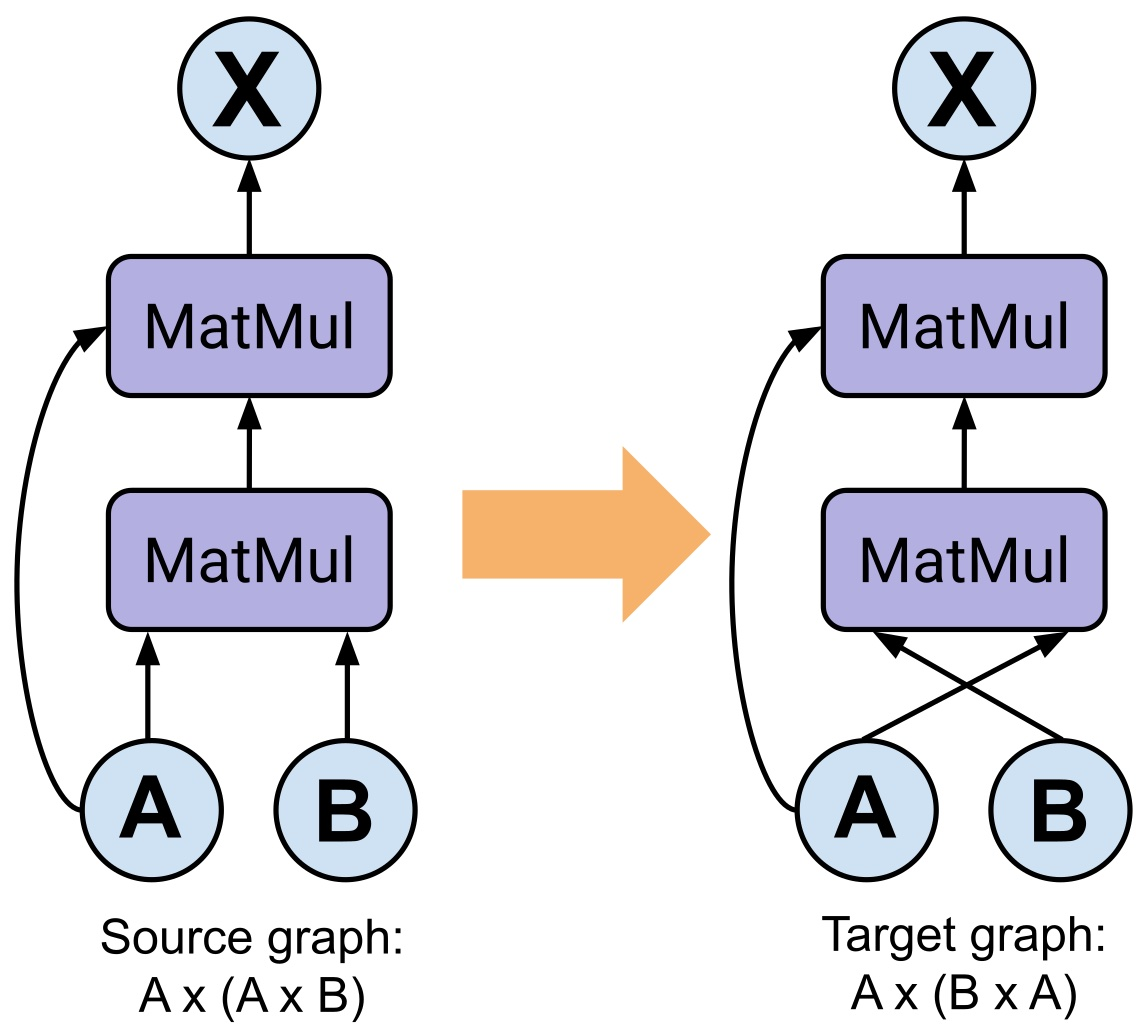
\includegraphics[height=3cm]{sections/3problem/images/rewrite1.jpg}%
      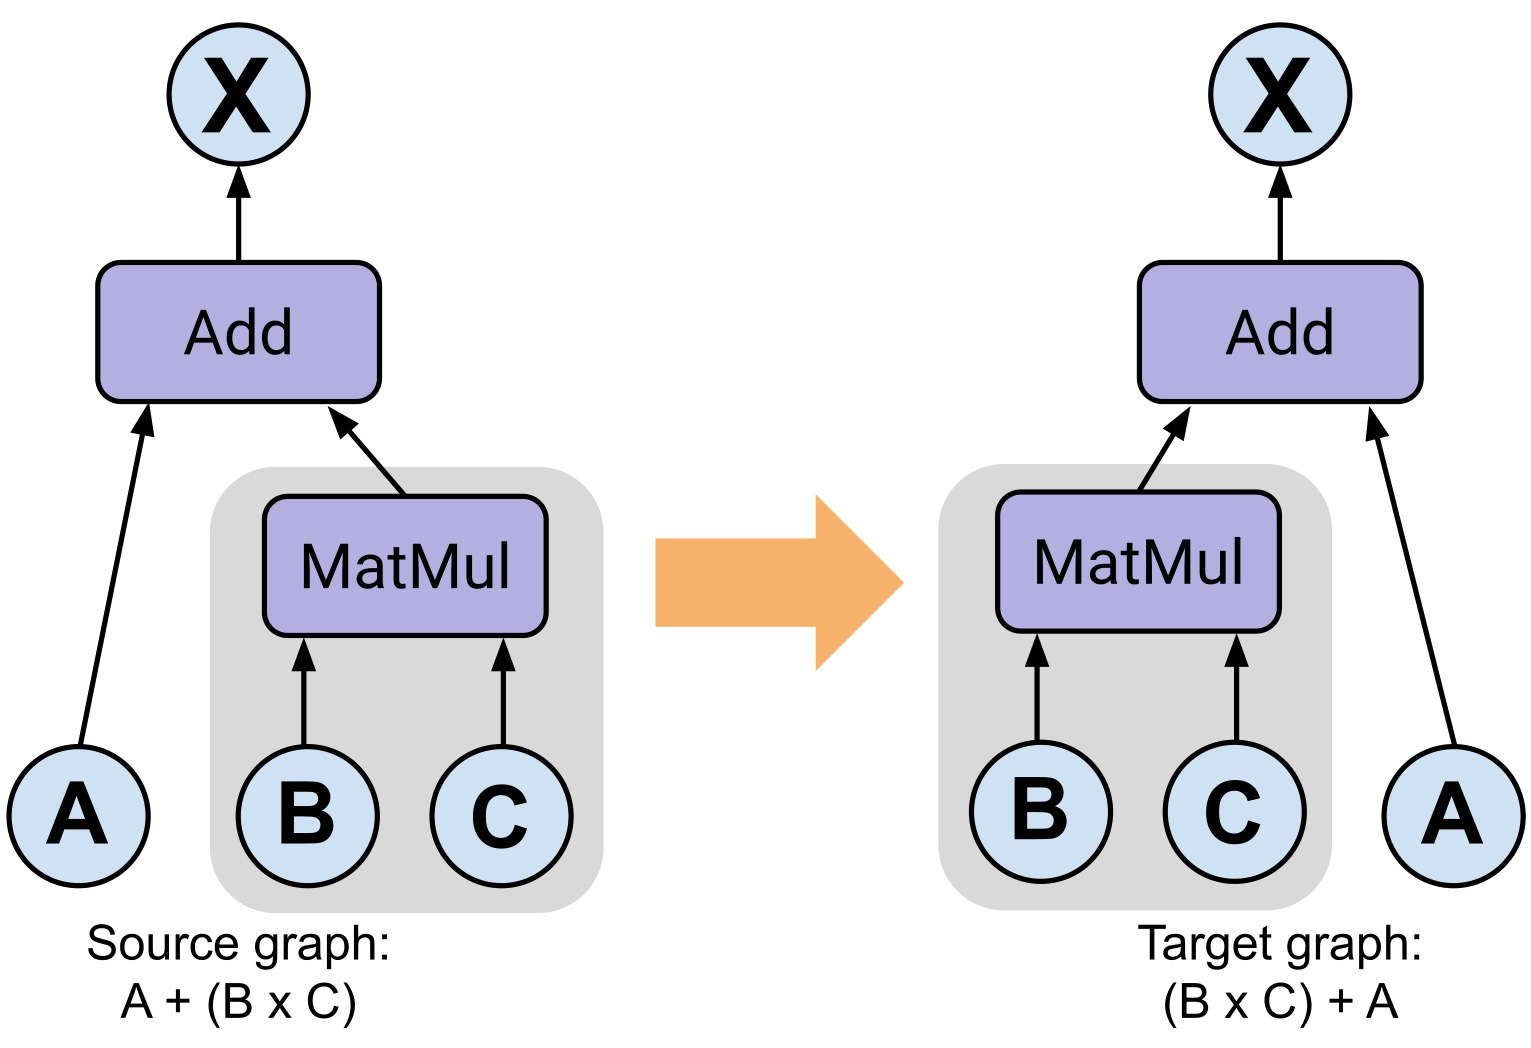
\includegraphics[height=3cm]{sections/3problem/images/rewrite2.jpg}%
    }%
  }
  \setlength{\twosubht}{\ht\twosubbox}
  
  % typeset
  \centering
  \subcaptionbox{Tensor renaming substitution \label{fig:problem:rewrite-graph1}}{
    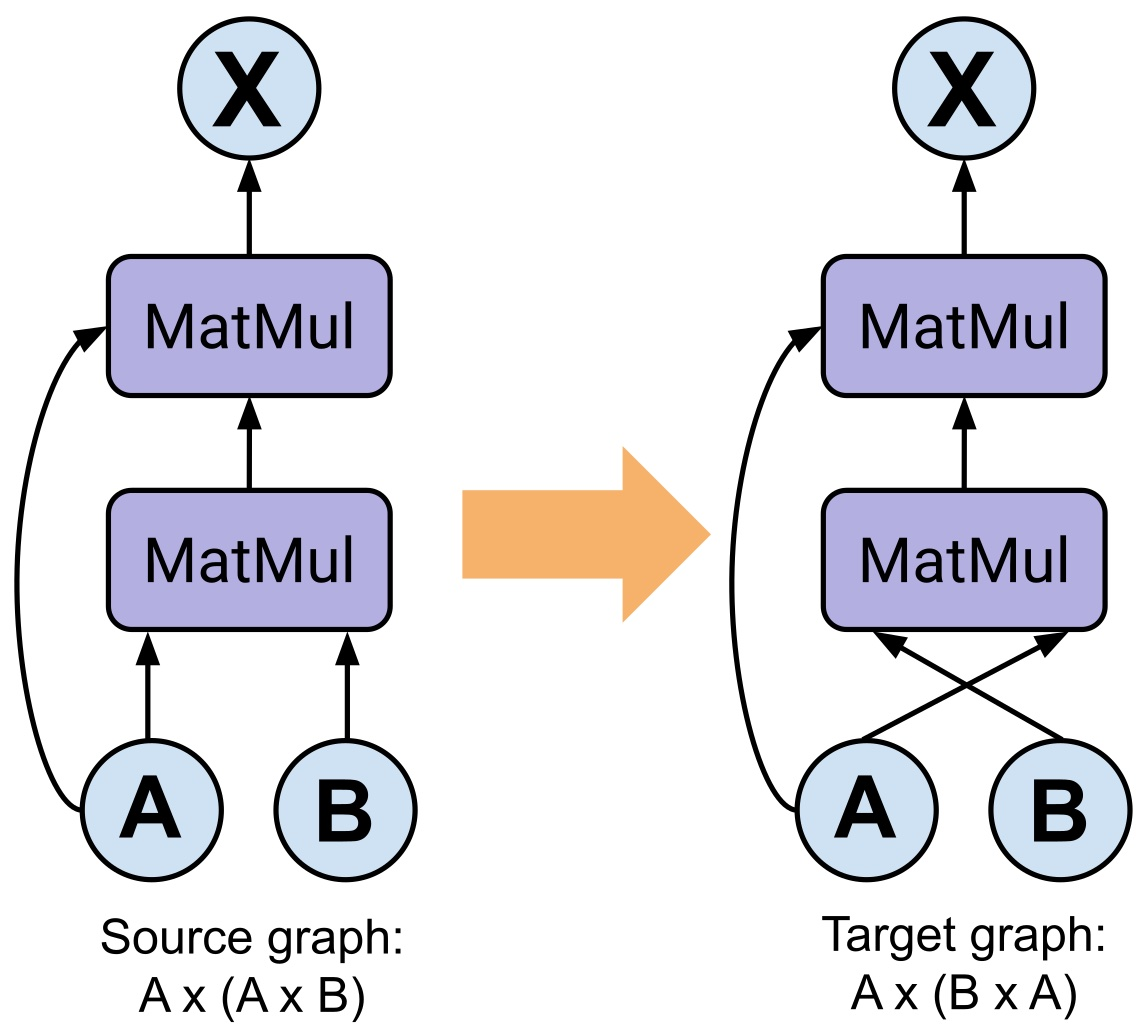
\includegraphics[height=\twosubht]{sections/3problem/images/rewrite1.jpg}
  }\quad
  \subcaptionbox{Common subgraph substitution \label{fig:problem:rewrite-graph2}}{
    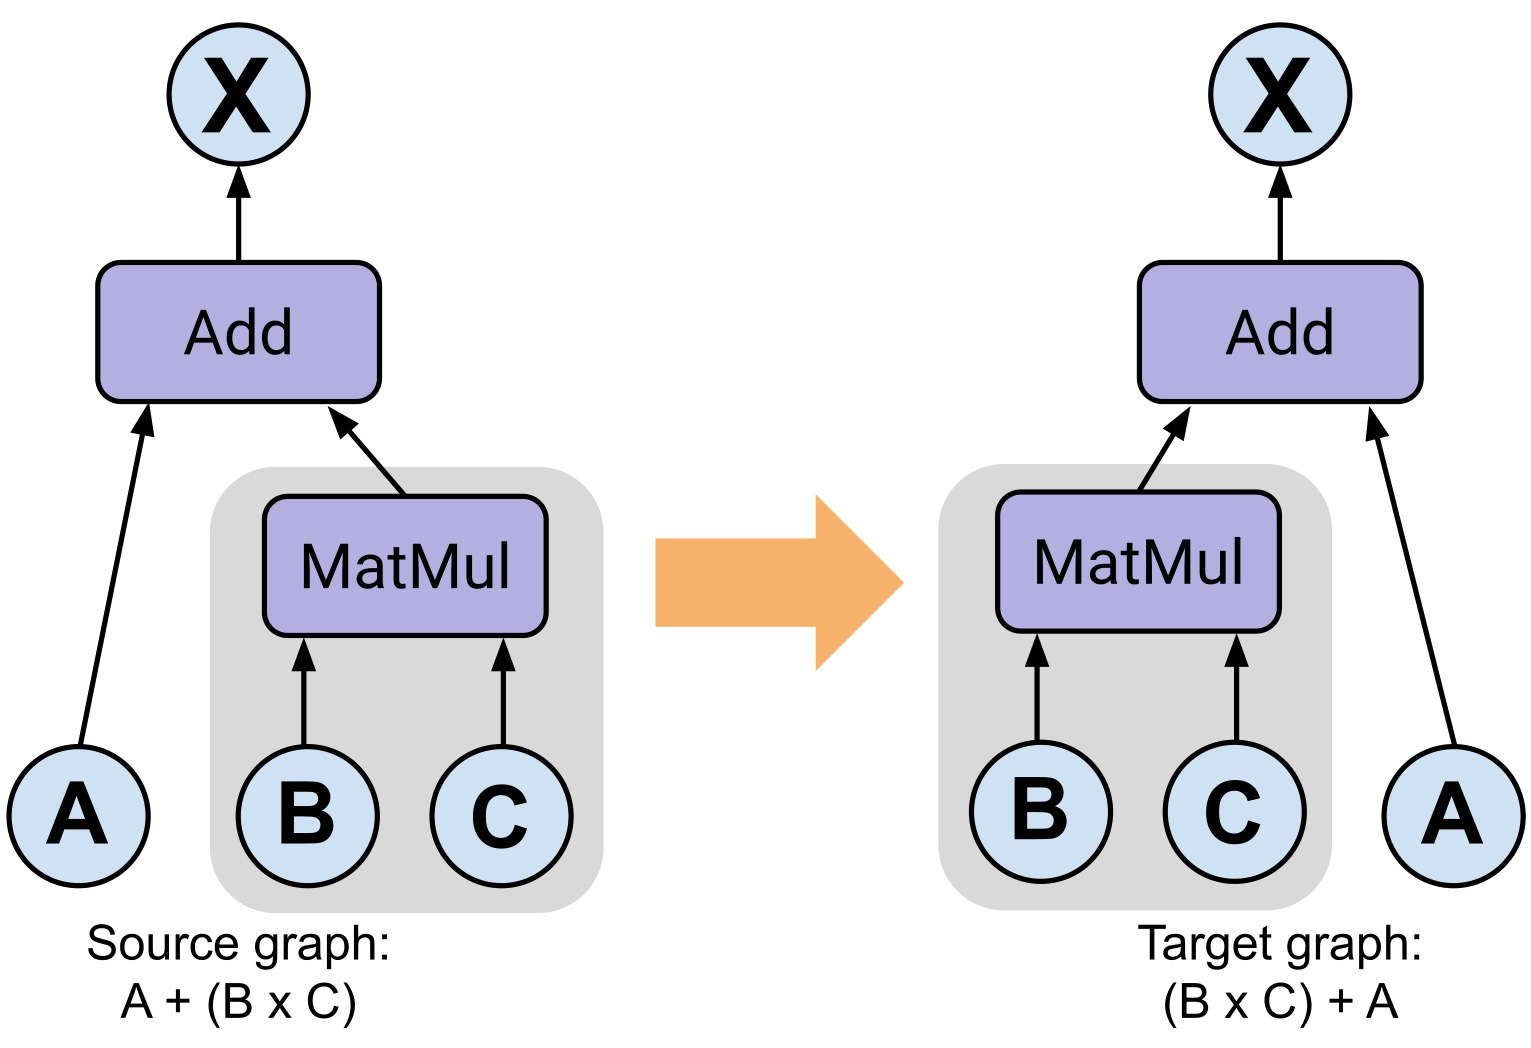
\includegraphics[height=\twosubht]{sections/3problem/images/rewrite2.jpg}
  }
  \caption{Two examples of trivial graph substitutions that does not impact the overall runtime of the computation graph}
\end{figure}

In this work, we take the same approach as that of TASO and automatically generate the candidate graphs. We perform this as an offline step as it requires a large amount of computation to both generate and verify the candidate substitutions. To place an upper bound on the computation, we limit the input tensor size to a maximum of 4x4x4x4 when verifying the candidate substitutions. Following the generation and verification steps, we prune the collection to remove substitutions that are considered trivial and as such would not impact runtime. For example, trivial substitutions include input tensor renaming and common subgraphs, we show both techniques diagrammatically in Figure \ref{fig:problem:rewrite-graph1} and \ref{fig:problem:rewrite-graph2} respectively.

\subsection{Baselines}

- Cost-based backtracking algorithm

- Estimation of runtime characteristics for each tensor op --> imperfect estimation

- Using real runtime is difficult as it takes longer to simulate and large variation in measurements between runs

\section{Reinforcement Learning formulation}

\subsection{System environment}

- Use TASO backend as the foundation for the system environment

- It has the ability to apply a specified transformation to the dataflow graph and return the transformed graph

- RL environments only need one function ``step'' that takes some action, applies the action to the environments internal state and returns the updated state

- Rewards are the TASO estimation of the runtime, we modified TASO to extract more detailed runtime measurements for performing reward engineering (ref chapter)

\subsection{State-Action space}

\subsection{Reward determination}

- Runtime difference

- Inclusion of detailed measurements

- Real-time measurements instead of estimated?

- Look up research on RL rewards (what makes a good reward signal)
